% !TEX root =  journal_main.tex

\section{Package options}
\begin{itemize}
	\item \verb|\usepackage{l16cn}|: default
	\item \verb|\usepackage[nopic]{l16cn}|: hide pictures (for faster compilation)
	\item \verb|\usepackage[nohl]{l16cn}|: hide highlights
	\item \verb|\usepackage[draft]{l16cn}|: add ``Confidential'' watermark
\end{itemize}

\section{File structure}
\begin{itemize}
	\item Main file: \verb|journal_main.tex|
	\item Sub-files:
	\begin{itemize}
		\item Abstract: \verb|abstract.tex|
		\item Glossary: \verb|definitions.tex|
		\item Bibliography: \verb|references.bib|
		\item Main text: \verb|text.tex|
	\end{itemize}
\end{itemize}

\section{Notation}
\verb|definitions.tex| contains all the 
definitions, acronyms, and notations.
Use \verb|\gls{ }| for
repeated glossary, acronym, and notation items, 
e.g.,~use \verb|\gls{abm}| for the first time,
you get ``\gls{abm}.'' Use it again, you get ``\gls{abm}.''
Similarly, you can use it on glossary items 
(e.g.,~use \verb|\glspl{al}| for plural ``\glspl{al}'')
and mathematical notations 
(e.g.,~use \verb|\gls{state}| or \verb|$\gls{state}$|
for \gls{state}).

\section{Multi-line equation}
Proper way to handle multi-line equations:
\begin{verbatim}
\begin{equation}
  \begin{aligned}
    x(t+1)&=Ax(t)+Bu(t)+\omega(t),\\
    y(t)&=Cx(t)+Du(t)+\nu(t).
  \end{aligned}
\end{equation}
\end{verbatim}
See output:
\begin{equation}
  \begin{aligned}
    x(t+1)&=Ax(t)+Bu(t)+\omega(t),\\
    y(t)&=Cx(t)+Du(t)+\nu(t).
  \end{aligned}
\end{equation}

\section{Figure}

Insert figure (below) and hide figure with the \verb|nopic| option.

\begin{figure}[h!]
   \centering
   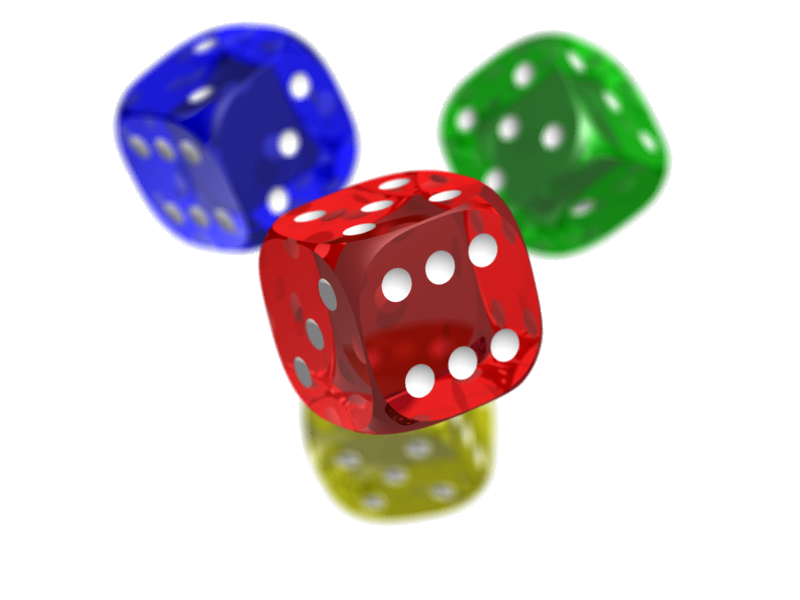
\includegraphics
   	[width=0.5\linewidth]{figs/dice.png}
   \caption{Dice}
   \label{fig:dice}
\end{figure}

\begin{verbatim}
\begin{figure}[htbp]
   \centering
   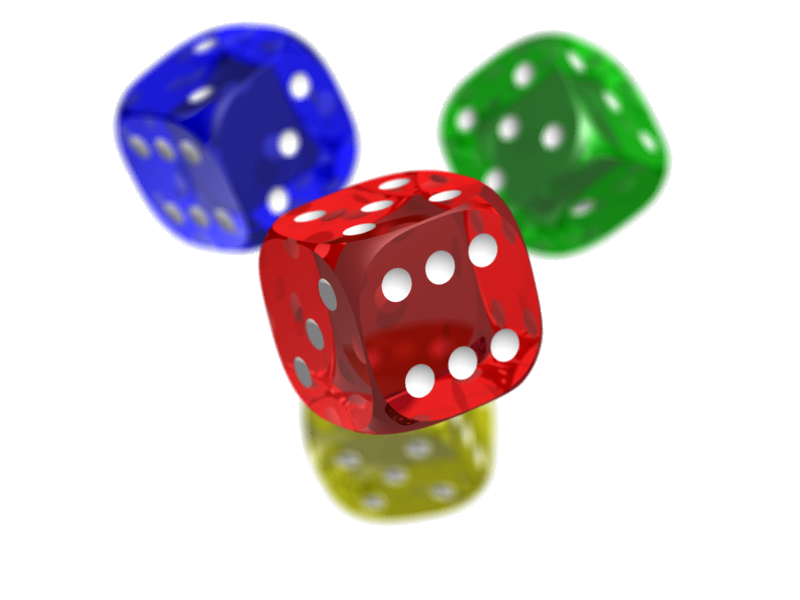
\includegraphics
   	[width=\linewidth]{figs/dice.png}
   \caption{Dice}
   \label{fig:dice}
\end{figure}
\end{verbatim}

\section{Highlight}
You can \hl{highlight} certain words with the \verb|\hl{ }| code. 
To hide the highlight, use the \verb|nohl| package option.


\section{Citation} 
\verb|references.bib| contains all the references.
Use \verb|\cite{}| for journal 
and \verb|\citep{}| for book.
For instance, \verb|\cite{galton1907vox}|
would return a numbered citation like this: \cite{galton1907vox}.
Numbered citations should be good for most journals.

\section{Root} Insert the following at the beginning
of every sub-file (replace \verb|<main file name>|)
with the main file name you use:
\begin{verbatim}
	% !TEX root =  <main file name>.tex
\end{verbatim}
For instance, if your main file is \verb|journal_main.tex|,
write the following at the first line of every sub-file:
\begin{verbatim}
	% !TEX root =  journal_main.tex
\end{verbatim}













